\documentclass[8pt,a4paper,compress,handout]{beamer}

\usepackage{/home/siyer/lib/slides}

\title{Input and Output}
\date{}
\RequirePackage{makecell}

\begin{document}
\begin{frame}
\hfill
\begin{minipage}{150pt}
\begin{flushright}
\tiny \emph{The most important property of a program is whether it accomplishes the intention of its user.}

\smallskip

- C. A. R. HOARE
\end{flushright}
\end{minipage}
\vfill
\titlepage
\end{frame}

\begin{frame}
\frametitle{Outline}
\tableofcontents
\end{frame}

\section{Input and Output}
\begin{frame}[fragile]
\begin{center}
\begin{tikzpicture}
\begin{scope}[->,xshift=-7.5cm,yshift=-5cm,thin,
	   node distance=1.6cm,on grid,>=stealth,
  	   block1/.style={rectangle,draw,align=center},
	   block2/.style={rectangle,align=center}]
\node [block2] (1) {input};
\node [block1] (2) [right=of 1] {\lstinline$my_program.py$};
\node [block2] (3) [right=of 2] {output};
\path (1) edge node [above] {} (2);
\path (2) edge node [above] {} (3);
\end{scope}
\end{tikzpicture}
\end{center}

\bigskip

\textbf{Input}
\begin{itemize}
\item Command-line input: The mechanism we have been using to provide
input values to our programs. We list them after the program name and access them using the \lstinline{sys.argv} list within the program. 
\item Standard input: Makes it possible to write programs that
process arbitrary amounts of input and to interact with the programs.
\item File input: Makes it possible to write programs that process multiple input streams.
\end{itemize}

\bigskip

\textbf{Output}
\begin{itemize}
\item Standard output: The mechanism we have been using to print output from our programs to the terminal window. We use methods such as \lstinline{stdio.write()} and \lstinline{stdio.writeln()}.
\item Standard drawing: Makes it possible to work with graphical representations of images.
\item Standard audio: Makes it possible to write programs that create sound.
\item File output: Makes it possible to write programs that process multiple output streams.
\end{itemize}
\end{frame}

\begin{frame}[fragile]
\begin{framed}
\tiny randomseq.py: Accept an integer command-line argument $n$. Write to standard output a random sequence of $n$ floats in the range $[0, 1)$.
\end{framed}

\begin{lstlisting}[language=Python]
import random
import stdio
import sys

n = int(sys.argv[1])
for i in range(n):
    stdio.writeln(random.random())
\end{lstlisting}

\begin{lstlisting}[language={}]
$ python randomseq.py 10
0.534835410847
0.249397020334
0.0460440369486
0.608142728098
0.686734322334
0.508728644023
0.831805280108
0.474190147291
0.89541446225
0.671581101113
\end{lstlisting}
\end{frame}

\section{Standard Output}
\begin{frame}[fragile]
API for the \lstinline{stdio} module relevant to standard output:
\begin{center}
\begin{tabular}{cc}
function call & description \\ \hline
\lstinline$stdio.write(x)$ & write $x$ to standard output \\
\lstinline$stdio.writeln(x)$ & write $x$ to standard output, followed by a newline \\
\lstinline$stdio.writef(fmt, arg1, ...)$ & \makecell{write the arguments $arg_1, \dots$ to standard output \\ as specified by the format string $fmt$} \\
\end{tabular} 
\end{center}

\bigskip

Formatted writing: In its simplest form, \lstinline{stdio.writef()} takes two arguments. The first argument is a format string that describes how to convert the second argument into a string for output.  For example, 
\begin{lstlisting}[language=Python]
stdio.writef('pi is approximately %.2f.\n', math.pi)
\end{lstlisting}
writes the output
\begin{lstlisting}[language={}]
pi is approximately 3.14.
\end{lstlisting}

\bigskip

The \lstinline{stdio.writef()} function can take more than two arguments.
In this case, the format string will have a format specifier for each additional argument, perhaps separated by other characters to pass through to the output. For example, 
\begin{lstlisting}[language=Python]
stdio.writef('The %dth decimal digit of %.10f is %d.\n', 5, math.pi, 9)
\end{lstlisting}
writes the output
\begin{lstlisting}[language={}]
The 5th decimal digit of 3.1415926536 is 9.
\end{lstlisting}
\end{frame}

\section{Standard Input}
\begin{frame}[fragile]
The \emph{standard input stream} is an abstract data stream that may be empty or may contain a sequence of values separated by whitespace. 

\bigskip

The end of the input stream is marked by the end-of-file (EOF) character, specified using \lstinline$<ctrl-d>$ or \lstinline$<ctrl-z>$. 

\bigskip

The \lstinline{stdio} module also supports reading from standard input stream.

\bigskip

A program that reads from standard input stream consumes the values, i.e., it cannot back up and read them again.
\end{frame}

\begin{frame}[fragile]
API for the \lstinline$stdio$ module relevant to standard input:
\begin{center}
\begin{tabular}{cc}
function call & description \\ \hline
\lstinline$stdio.isEmpty()$ & is the standard input empty (or only whitespace)? \\
\lstinline$stdio.readInt()$ & read a token, convert it to an integer, and return it \\
\lstinline$stdio.readFloat()$ & read a token, convert it to a float, and return it \\
\lstinline$stdio.readBool()$ & read a token, convert it to a boolean, and return it \\
\lstinline$stdio.readString()$ & read a token and return it as a string \\
\lstinline$stdio.hasNextLine()$ & does standard input have a next line? \\
\lstinline$stdio.readLine()$ & read the next line and return it as a string \\
\lstinline$stdio.readAll()$ & read all remaining input and return it as a string \\
\lstinline$stdio.readAllInts()$ & read all remaining tokens and return them as a list of integers \\
\lstinline$stdio.readAllFloats()$ & read all remaining tokens and return them as a list of floats \\
\lstinline$stdio.readAllBools()$ & read all remaining tokens and return them as a list of booleans \\
\lstinline$stdio.readAllStrings()$ & read all remaining tokens and return them as a list of strings \\
\lstinline$stdio.readAllLines()$ & read all remaining lines and return them as a list of strings
\end{tabular} 
\end{center}
\end{frame}

\begin{frame}[fragile]
\begin{framed}
\tiny twentyquestions.py: Generate a random integer. Repeatedly read user guesses from standard input. Write 'Too low' or 'Too high' to standard output, as appropriate, in response to each guess. Write 'You win!' and exit when the user's guess is correct.
\end{framed}

\begin{lstlisting}[language=Python]
import random
import stdio

RANGE = 1000000
secret = random.randrange(1, RANGE + 1)
stdio.write('I am thinking of a secret number between 1 and ')
stdio.writeln(RANGE)
guess = 0
while guess != secret:
    stdio.write('What is your guess? ')
    guess = stdio.readInt()
    if (guess < secret):
        stdio.writeln('Too low')
    elif (guess > secret):
        stdio.writeln('Too high')
    else:
        stdio.writeln('You win!')
\end{lstlisting}

\begin{lstlisting}[language={}]
$ python twentyquestions.py
I am thinking of a secret number between 1 and 1000000
What is your guess? 500000
Too low
What is your guess? 750000     
Too high
What is your guess? 625000
Too high
...
What is your guess? 501686
You win!
\end{lstlisting}

\end{frame}

\begin{frame}[fragile]
\begin{framed}
\tiny average.py: Read floats from the standard input stream until end-of-file. Write to standard output the average of those floats.
\end{framed}

\begin{lstlisting}[language=Python]
import stdio

total = 0.0
count = 0
while not stdio.isEmpty():
    value = stdio.readFloat()
    total += value
    count += 1
avg = total / count
stdio.writeln('Average is ' + str(avg))
\end{lstlisting}

\begin{lstlisting}[language={}]
$ python average.py
10.0 5.0 6.0
3.0
7.0 32.0
<ctrl-d>
Average is 10.5
\end{lstlisting}
\end{frame}

\section{Redirection and Piping}
\begin{frame}[fragile]
By adding the directive \lstinline{>} to the command that invokes a program, we can redirect its standard output to a file, either for permanent storage or for input to another program at a later time. For example: 
\begin{lstlisting}[language={}]
$ python randomseq.py 1000 > data.txt
$ head -5 data.txt 
0.12490675039
0.509198876091
0.224604151916
0.918194898729
0.296035502122
\end{lstlisting}

\bigskip

Similarly, by adding the directive \lstinline{<} to the command that invokes a program, we can redirect standard input so that \lstinline{stdio} reads data from a file instead of the terminal. For example:  
\begin{lstlisting}[language={}]
$ python average.py < data.txt
Average is 0.499379975213
\end{lstlisting}

\bigskip

The standard output of one program can be mapped to the standard input stream of another program using the (pipe) directive \lstinline{|}. For example:  
\begin{lstlisting}[language={}]
$ python randomseq.py 1000 | python average.py 
Average is 0.501346917807
$ python randomseq.py 1000 | python average.py | wc
      1       3      26
\end{lstlisting}
\end{frame}

\begin{frame}[fragile]
\begin{framed}
\tiny rangefilter.py: Accept integer command-line arguments $lo$ and $hi$. Read integers from standard input until end-of-file. Write to standard output each of those integers that is in the range $lo$ to $hi$, inclusive.
\end{framed}

\begin{lstlisting}[language=Python]
import stdio
import sys

lo = int(sys.argv[1])
hi = int(sys.argv[2])
while not stdio.isEmpty():
    value = stdio.readInt()
    if (value >= lo) and (value <= hi):
        stdio.write(str(value) + ' ')
stdio.writeln()
\end{lstlisting}

\begin{lstlisting}[language={}]
$ python rangefilter.py 100 400
358 1330 55 165 689 1014 3066 387 575 843 203 48 292 877 65 998
358 165 387 203 292
<ctrl-d>
$ seq 1 100 | shuf | python rangefilter.py 25 75
50 41 45 70 32 34 55 26 27 51 71 58 44 59 39 72 66 35 25 29 40 43 73 64 56 31 38 
65 69 46 54 30 62 67 57 48 68 74 36 42 37 52 53 33 75 47 28 60 63 49 61 
$ seq 1 1000 | shuf | python rangefilter.py 250 750 | wc -w
501
\end{lstlisting}
\end{frame}

\section{Standard Drawing}
\begin{frame}[fragile]
The \lstinline{stddraw} module provides an abstraction for producing drawings as output.

\bigskip

API for the \lstinline{stddraw} module (drawing functions):
\begin{center}
\begin{tabular}{cc}
function call & description \\ \hline
\lstinline$stddraw.line(x0, y0, x1, y1)$ & draw a line from $(x_0, y_0)$ to $(x_1, y_1)$ \\
\lstinline$stddraw.point(x, y)$ & draw a point at $(x, y)$ \\
\lstinline$stddraw.circle(x, y, r)$ & draw a circle of radius $r$ centered at $(x, y)$ \\
\lstinline$stddraw.filledCircle(x, y, r)$ & draw a filled circle of radius $r$ centered at $(x, y)$ \\
\lstinline$stddraw.square(x, y, r)$ & draw a $2r$-by-$2r$ square centered at $(x, y)$ \\
\lstinline$stddraw.filledSquare(x, y, r)$ & draw a filled $2r$-by-$2r$ square centered at $(x, y)$ \\
\lstinline$stddraw.rectangle(x, y, w, h)$ & \makecell{draw a $w$-by-$h$ rectangle \\ with lower left point at $(x, y)$} \\ 
\lstinline$stddraw.filledRectangle(x, y, w, h)$ & \makecell{draw a filled $w$-by-$h$ rectangle \\ with lower left point at $(x, y)$} \\
\lstinline$stddraw.polygon(x, y)$ & draw a polygon with coordinates $(x_i, y_i)$ \\
\lstinline$stddraw.filledPolygon(x, y)$ & draw a filled polygon with coordinates $(x_i, y_i)$ \\
\lstinline$stddraw.text(x, y, s)$ & draw a string $s$ at $(x, y)$ \\
\end{tabular} 
\end{center}
\end{frame}

\begin{frame}[fragile]
API for the \lstinline{stddraw} module (control functions):
\begin{center}
\begin{tabular}{cc}
function call & description \\ \hline
\lstinline$stddraw.setCanvasSize(w, h)$ & set canvas size to $w$-by-$h$ pixels \\
\lstinline$stddraw.setXscale(x0, x1)$ & set $x$-range of canvas to $x_0, x_1$ \\
\lstinline$stddraw.setYscale(y0, y1)$ & set $y$-range of canvas to $y_0, y_1$ \\
\lstinline$stddraw.setPenRadius(r)$ & set pen radius to $r$ \\
\lstinline$stddraw.setPenColor(c)$ & set pen color to $c$ \\
\lstinline$stddraw.setFontFamily(f)$ & set font family to $f$ \\
\lstinline$stddraw.setFontSize(s)$ & set font size to $s$ \\
\lstinline$stddraw.clear(c)$ & clear canvas by coloring every pixel with color $c$ \\
\lstinline$stddraw.show(t)$ & show the drawing on canvas and wait $t$ milliseconds \\
\lstinline$stddraw.save(f)$ & save canvas to file $f$ 
\end{tabular} 
\end{center}

\end{frame}

\begin{frame}[fragile]
\begin{framed}
\tiny plotfilter.py: Read $x$ and $y$ scales from standard input, and configure standard draw accordingly. Then read points from standard input until end-of-file, and plot them on standard draw.
\end{framed}

\begin{lstlisting}[language=Python]
import stddraw
import stdio

x0 = stdio.readFloat()
y0 = stdio.readFloat()
x1 = stdio.readFloat()
y1 = stdio.readFloat()
stddraw.setXscale(x0, x1)
stddraw.setYscale(y0, y1)
stddraw.setPenRadius(0.0)
while not stdio.isEmpty():
    x = stdio.readFloat()
    y = stdio.readFloat()
    stddraw.point(x, y)
stddraw.show()
\end{lstlisting}

\begin{minipage}{150pt}
\begin{lstlisting}[language={}]
$ head -5 usa.txt 
669905.0 247205.0 1244962.0 500000.0
 1097038.8890   245552.7780
 1103961.1110   247133.3330
 1104677.7780   247205.5560
 1108586.1110   249238.8890
$ python plotfilter.py < usa.txt
\end{lstlisting}
\end{minipage}%
\begin{minipage}{150pt}
\hfill 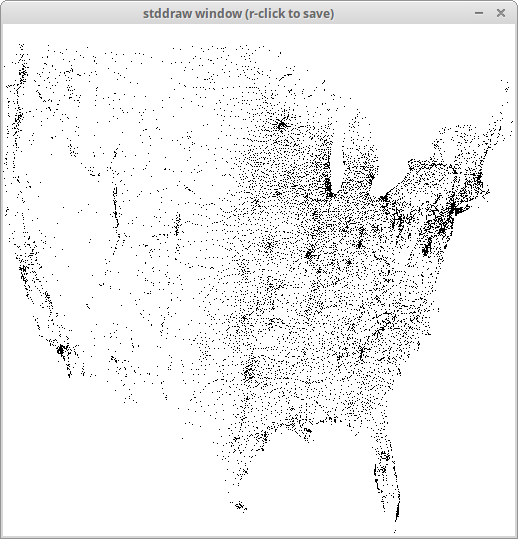
\includegraphics[scale=0.18]{figures/usa.png}
\end{minipage}
\end{frame}

\begin{frame}[fragile]
\begin{framed}
\tiny bouncingball.py: Draw a bouncing ball to standard draw.
\end{framed}

\begin{lstlisting}[language=Python]
import stddraw

RADIUS = .05
DT = 20.0
stddraw.setXscale(-1.0, 1.0)
stddraw.setYscale(-1.0, 1.0)
rx = .480
ry = .860
vx = .015
vy = .023
while True:
    if abs(rx + vx) + RADIUS > 1.0:
        vx = -vx
    if abs(ry + vy) + RADIUS > 1.0:
        vy = -vy
    rx = rx + vx
    ry = ry + vy
    stddraw.clear(stddraw.WHITE)
    stddraw.filledCircle(rx, ry, RADIUS)
    stddraw.show(DT)
\end{lstlisting}

\begin{minipage}{150pt}
\begin{lstlisting}[language={}]
$ python bouncingball.py
\end{lstlisting}
\end{minipage}%
\begin{minipage}{150pt}
\hfill 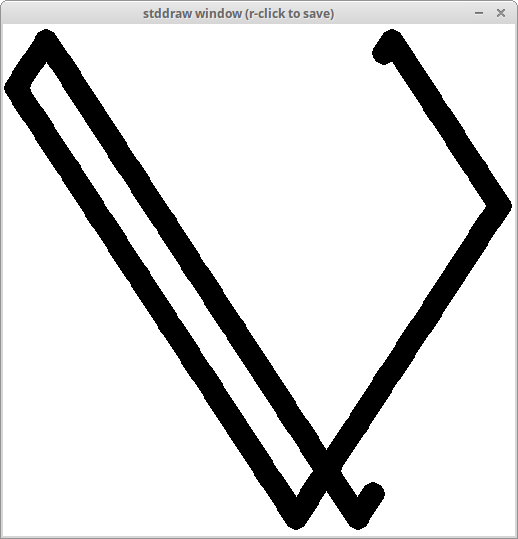
\includegraphics[scale=0.13]{figures/bouncing_ball.png}
\end{minipage}
\end{frame}

\section{Standard Audio}
\begin{frame}[fragile]
The \lstinline{stdaudio} module is an abstraction for playing, manipulating, and synthesizing sounds.

\bigskip

API for the \lstinline{stdaudio} module:
\begin{center}
\begin{tabular}{cc}
function call & description \\ \hline
\lstinline$stdaudio.playSamples(a)$ & play all sound samples in the array $a$ \\
\lstinline$stdaudio.playFile(f)$ & play all sound samples in the \lstinline$.wav$ file $f$ \\
\lstinline$stdaudio.playSample(s)$ & play the sound sample $s$ \\
\lstinline$stdaudio.save(f, a)$ & save the sound samples in array $a$ to the (\lstinline$.wav$) file $f$ \\
\lstinline$stdaudio.wait()$ & wait for the currently playing sound to finish
\end{tabular} 
\end{center}
\end{frame}

\begin{frame}[fragile]
\begin{framed}
\tiny playthattune.py: Read sound samples from standard input, and play the sound to standard audio.
\end{framed}

\begin{lstlisting}[language=Python]
import math
import stdarray
import stdaudio
import stdio

SPS = 44100
CONCERT_A = 440.0
NOTES_ON_SCALE = 12.0
while not stdio.isEmpty():
    pitch = stdio.readInt()
    duration = stdio.readFloat()
    hz = CONCERT_A * (2.0 ** (pitch / NOTES_ON_SCALE))
    n = int(SPS * duration)
    note = stdarray.create1D(n + 1, 0.0)
    for i in range(n + 1):
        note[i] = math.sin(2.0 * math.pi * i * hz / SPS)
    stdaudio.playSamples(note)
stdaudio.wait()
\end{lstlisting}

\begin{minipage}{150pt}
\begin{lstlisting}[language={}]
$ head -5 elise.txt
7 .125 
6 .125 
7 .125 
6 .125 
7 .125 
$ python playthattune.py < elise.txt
\end{lstlisting}
\end{minipage}%
\begin{minipage}{150pt}
\hfill 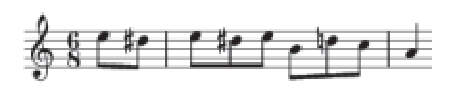
\includegraphics[scale=0.5]{figures/furelise.pdf}
\end{minipage}
\end{frame}
\end{document}
